\chapter{Respiração celular e fermentação}\label{ch:b1:respiration-fermentation}

Um frasco de levedura em solução açucarada com o ar excluído borbulha
dióxido de carbono e transforma o açúcar em álcool; deixe o ar entrar e
o borbulhar diminui, o álcool cessa, e a levedura cresce dez vezes mais
rápido com o mesmo açúcar. Pasteur viu isso em 1861 e não conseguiu
explicar; a explicação levou um século e atravessa este capítulo
inteiro. O oxigênio permite a uma \omterm{def:b1:cell-unit-of-life:cell}{célula} extrair da glicose quinze vezes
a energia que ela consegue sem ele, e o faz passando os elétrons do
açúcar por uma cadeia de transportadores até o oxigênio, bombeando
prótons através de uma membrana enquanto eles caem, e deixando os
prótons voltarem por uma turbina que fabrica \omterm{def:b1:water-small-molecules:atp}{ATP}. Este capítulo descreve
a \omterm{def:b1:respiration-fermentation:glycolysis}{glicólise}, o \omterm{def:b1:respiration-fermentation:krebs}{ciclo de Krebs}, a \omterm{def:b1:respiration-fermentation:chain}{cadeia respiratória} e o acoplamento
quimiosmótico dela, as \omterm{def:b1:respiration-fermentation:fermentation}{fermentações} que dispensam o oxigênio, e a
queima de \omterm{def:b1:lipids:triglyceride}{gorduras} e \omterm{def:b1:proteins:peptide}{proteínas} pela mesma maquinaria.

\section{A oxidação da glicose}

\begin{proposition}[A reação global e as etapas dela]\label{prop:b1:respiration-fermentation:overview}
\index{respiração celular}
A oxidação completa da glicose,
\[
\mathrm{C_6H_{12}O_6} + 6\,\mathrm{O_2} \to 6\,\mathrm{CO_2} + 6\,\mathrm{H_2O},
\qquad \Delta G^{\circ\prime} = \qty{-2870}{kJ/mol},
\]
é realizada em três etapas que nunca deixam os elétrons encontrarem o
oxigênio diretamente. A \emph{\omterm{def:b1:respiration-fermentation:glycolysis}{glicólise}}, no \omterm{def:b1:eukaryotic-cell:organelle}{citosol}, parte a glicose em
dois piruvatos e rende 2 \omterm{def:b1:water-small-molecules:atp}{ATP} e 2 NADH. A \emph{oxidação do piruvato e o
\omterm{def:b1:respiration-fermentation:krebs}{ciclo de Krebs}}, na \omterm{def:b1:eukaryotic-cell:mitochondrion}{matriz mitocondrial}, oxidam o piruvato a
$\mathrm{CO_2}$, carregando os elétrons em 8 NADH e 2
$\mathrm{FADH_2}$ e fabricando 2 GTP. A \emph{fosforilação oxidativa},
na membrana mitocondrial interna, passa esses elétrons ao oxigênio por
uma cadeia de transportadores que bombeia prótons, e o gradiente de
prótons move a síntese de cerca de 26 \omterm{def:b1:water-small-molecules:atp}{ATP}. Ao todo, uns 30 \omterm{def:b1:water-small-molecules:atp}{ATP} por
glicose: cerca de metade da \omterm{prop:b1:water-small-molecules:gibbs}{energia livre} de combustão capturada, e o
resto liberado como calor.
\end{proposition}

\begin{definition}[Transportadores de elétrons]\label{def:b1:respiration-fermentation:carriers}
\index{NAD}\index{FAD}
O \emph{$\mathrm{NAD^+}$} (dinucleotídeo de nicotinamida e adenina)
aceita dois elétrons e um próton de um \omterm{def:b1:enzymes:enzyme}{substrato} e vira NADH; o
\emph{FAD} aceita dois elétrons e dois prótons e vira $\mathrm{FADH_2}$.
Os dois são \omterm{def:b1:enzymes:enzyme}{coenzimas} de desidrogenases, e os dois são reciclados:
reduzidos pelo catabolismo, reoxidados pela \omterm{def:b1:respiration-fermentation:chain}{cadeia respiratória}. Uma
\omterm{def:b1:cell-unit-of-life:cell}{célula} contém apenas micromols deles, que se renovam milhares de vezes
por hora. Os potenciais redox deles, $E'_0 = \qty{-0.32}{V}$ para o par
$\mathrm{NAD^+}/\mathrm{NADH}$, os põem muito abaixo do oxigênio
($\qty{+0.82}{V}$): cada par de elétrons que o NADH entrega ao oxigênio
libera $\Delta G^{\circ\prime} = -2F\Delta E =
\qty{-220}{kJ/mol}$, o bastante para mais de quatro \omterm{def:b1:water-small-molecules:atp}{ATP}.
\end{definition}

\begin{omfigure}
\begin{tikzpicture}[font=\footnotesize, >=Stealth, line cap=round,
  st/.style={draw, thick, rounded corners=4pt, minimum height=9mm, text width=30mm, align=center, fill=white}]
  \node[st, fill=omDef!12] (gly) at (0,0) {\textbf{glicólise}\\ citosol\\ glicose $\to$ 2 piruvatos};
  \node[st, fill=omProp!12] (krebs) at (5.4,0) {\textbf{oxidação do piruvato}\\ \textbf{+ ciclo de Krebs}\\ matriz; 2 piruvatos $\to$ 6 $\mathrm{CO_2}$};
  \node[st, fill=omThm!12] (ox) at (10.8,0) {\textbf{fosforilação}\\ \textbf{oxidativa}\\ membrana interna; $\mathrm{O_2} \to \mathrm{H_2O}$};
  \draw[->, very thick] (gly) -- (krebs) node[midway, above, font=\scriptsize] {2 piruvatos};
  \draw[->, very thick] (krebs) -- (ox) node[midway, above, align=center, font=\scriptsize] {8 NADH\\ 2 $\mathrm{FADH_2}$};
  \draw[->, very thick] (gly.north) .. controls (0,1.8) and (10.8,1.8) .. (ox.north) node[pos=0.5, above] {2 NADH};
  \node[anchor=north, omExo!70!black] at (gly.south) {2 ATP};
  \node[anchor=north, omExo!70!black] at (krebs.south) {2 GTP};
  \node[anchor=north, omExo!70!black] at (ox.south) {$\approx$ 26 ATP};
  \node[anchor=north, align=center, gray] at (5.4,-1.75) {total $\approx$ 30 ATP por glicose, cerca de metade dos \qty{2870}{kJ/mol}};
\end{tikzpicture}

{\small As três etapas da respiração. A \omterm{def:b1:respiration-fermentation:glycolysis}{glicólise} e o \omterm{def:b1:respiration-fermentation:krebs}{ciclo de Krebs}
retiram os elétrons da glicose e os põem no NADH e no
$\mathrm{FADH_2}$; a fosforilação oxidativa os converte em dinheiro.}
\end{omfigure}

\section{A glicólise}

\begin{definition}[Glicólise]\label{def:b1:respiration-fermentation:glycolysis}
\index{glicólise}
A \emph{glicólise} é uma sequência de dez reações enzimáticas no \omterm{def:b1:eukaryotic-cell:organelle}{citosol}
que converte uma glicose (C6) em dois \emph{piruvatos} (C3). Na
\emph{fase de investimento} dois \omterm{def:b1:water-small-molecules:atp}{ATP} são gastos para fosforilar o
açúcar (a hexoquinase e depois a \emph{fosfofrutoquinase}, PFK), e o
difosfato de seis carbonos é partido em dois fosfatos de três carbonos.
Na \emph{fase de retorno} cada triose é oxidada pelo $\mathrm{NAD^+}$ (a
única oxidação da glicólise) e os fosfatos dela são transferidos ao ADP
por \emph{fosforilação em nível de substrato}\index{fosforilação em nível de substrato}
--- um fosfato entregue diretamente de um intermediário rico em energia
ao ADP, sem membrana nem oxigênio envolvidos. O balanço:
\[
\text{glicose} + 2\,\mathrm{NAD^+} + 2\,\mathrm{ADP} + 2\,\mathrm{P_i}
\to 2\,\text{piruvato} + 2\,\mathrm{NADH} + 2\,\mathrm{H^+} + 2\,\mathrm{ATP} + 2\,\mathrm{H_2O} .
\]
Ela não precisa de oxigênio; é a via mais antiga e mais universal do
metabolismo.
\end{definition}

\begin{omfigure}
\begin{tikzpicture}[font=\footnotesize, >=Stealth, line cap=round,
  m/.style={draw, thick, rounded corners=3pt, minimum height=7mm, align=center, fill=omDef!10, inner sep=3pt},
  lab/.style={font=\scriptsize}]
  \node[m] (glc) at (0,0) {glicose};
  \node[m] (g6p) at (3.4,0) {glicose-6-P};
  \node[m] (f6p) at (7.0,0) {frutose-6-P};
  \node[m] (fbp) at (10.8,0) {frutose-1,6-bisP};
  \node[m, fill=omProp!12] (g3p) at (10.8,-2.2) {2 gliceraldeído-3-P};
  \node[m, fill=omProp!12] (bpg) at (5.6,-2.2) {2 1,3-bisfosfoglicerato};
  \node[m, fill=omProp!12] (pep) at (5.6,-4.2) {2 fosfoenolpiruvato};
  \node[m, fill=omProp!12] (pyr) at (1.0,-4.2) {2 piruvato};
  \draw[->, thick] (glc) -- (g6p) node[midway, above=3pt, omThm, font=\scriptsize] {ATP} node[midway, below=3pt, lab] {hexoquinase};
  \draw[->, thick] (g6p) -- (f6p);
  \draw[->, thick] (f6p) -- (fbp) node[midway, above=3pt, omThm, font=\scriptsize] {ATP};
  \node[lab, anchor=north] at (8.9,-0.42) {PFK (regulada)};
  \draw[->, thick] (fbp) -- (g3p) node[midway, right, lab] {partida em duas trioses};
  \draw[->, thick] (g3p) -- (bpg);
  \node[lab, anchor=south, omExo!70!black] at (8.6,-1.78) {2 $\mathrm{NAD^+} \to$ 2 NADH};
  \node[lab, anchor=north] at (8.6,-2.62) {oxidação};
  \draw[->, thick] (bpg) -- (pep) node[midway, right, omExo!70!black] {2 ATP};
  \draw[->, thick] (pep) -- (pyr) node[midway, above, omExo!70!black] {2 ATP};
  \node[anchor=north west, align=left, gray] at (-0.6,-5.0) {investimento: $-2$ ATP (caixas azuis) \quad retorno: $+4$ ATP, $+2$ NADH (caixas laranja)\\ líquido: $+2$ ATP, $+2$ NADH};
\end{tikzpicture}

{\small A \omterm{def:b1:respiration-fermentation:glycolysis}{glicólise} em linhas gerais. Dois \omterm{def:b1:water-small-molecules:atp}{ATP} são gastos para construir
um difosfato de seis carbonos, que se parte em duas trioses; a oxidação
delas e duas \omterm{def:b1:respiration-fermentation:glycolysis}{fosforilações em nível de substrato} devolvem, cada par,
quatro \omterm{def:b1:water-small-molecules:atp}{ATP} e dois NADH. A fosfofrutoquinase é a válvula de controle da
via.}
\end{omfigure}

\begin{proposition}[Controle na fosfofrutoquinase]\label{prop:b1:respiration-fermentation:pfk}
A PFK, a primeira etapa irreversível comprometida com a \omterm{def:b1:respiration-fermentation:glycolysis}{glicólise}, é uma
\omterm{def:b1:enzymes:allosteric}{enzima alostérica} (\cref{ch:b1:enzymes}) inibida pelo \omterm{def:b1:water-small-molecules:atp}{ATP} e pelo citrato
--- os sinais de que a energia e o combustível do \omterm{def:b1:respiration-fermentation:krebs}{ciclo de Krebs} estão
abundantes --- e ativada pelo AMP e pelo ADP, os sinais de que não
estão. Quando o \omterm{def:b1:water-small-molecules:atp}{ATP} está alto, o fluxo pela \omterm{def:b1:respiration-fermentation:glycolysis}{glicólise} cai em segundos;
quando a \omterm{def:b1:cell-unit-of-life:cell}{célula} gasta \omterm{def:b1:water-small-molecules:atp}{ATP}, o AMP sobe bruscamente (pela adenilato
quinase, $2\,\mathrm{ADP} \rightleftharpoons \mathrm{ATP} + \mathrm{AMP}$)
e a PFK se abre. A \emph{carga energética} da \omterm{def:b1:cell-unit-of-life:cell}{célula}
regula a via que a preenche.
\end{proposition}

\section{Oxidação do piruvato e ciclo de Krebs}

\begin{definition}[Piruvato-desidrogenase, acetil-CoA]\label{def:b1:respiration-fermentation:pdh}
O piruvato entra na \omterm{def:b1:eukaryotic-cell:mitochondrion}{mitocôndria} e é oxidado pelo complexo
\emph{piruvato-desidrogenase} a \emph{acetil-CoA}\index{acetil-CoA} ---
um grupo acetila de dois carbonos carregado pela \omterm{def:b1:enzymes:enzyme}{coenzima} A
(\cref{ch:b1:nucleic-acids}) numa ligação tioéster rica em energia ---,
liberando um $\mathrm{CO_2}$ e um NADH. O acetil-CoA é a entrada comum
de todos os combustíveis no ciclo: os \omterm{def:b1:carbohydrates:monosaccharide}{carboidratos} pelo piruvato, as
\omterm{def:b1:lipids:triglyceride}{gorduras} pela $\beta$-oxidação, e muitos \omterm{def:b1:proteins:aminoacid}{aminoácidos} diretamente.
\end{definition}

\begin{definition}[O ciclo de Krebs]\label{def:b1:respiration-fermentation:krebs}
\index{ciclo de Krebs}\index{ciclo do ácido cítrico}
O \emph{ciclo de Krebs} (ciclo do ácido cítrico), na \omterm{def:b1:eukaryotic-cell:mitochondrion}{matriz
mitocondrial}, condensa o \omterm{def:b1:respiration-fermentation:pdh}{acetil-CoA} (C2) com o oxaloacetato (C4) em
citrato (C6) e, em oito etapas, oxida os dois carbonos a $\mathrm{CO_2}$
enquanto regenera o oxaloacetato. Por grupo acetila: 3 NADH, 1
$\mathrm{FADH_2}$, 1 GTP (por \omterm{def:b1:respiration-fermentation:glycolysis}{fosforilação em nível de substrato}) e 2
$\mathrm{CO_2}$. Por glicose (dois acetilas): 6 NADH, 2
$\mathrm{FADH_2}$, 2 GTP, 4 $\mathrm{CO_2}$ --- que, com os 2
$\mathrm{CO_2}$ da piruvato-desidrogenase, dão os seis da equação
global. Nenhum oxigênio é consumido no ciclo em si; ele só funciona
enquanto a \omterm{def:b1:respiration-fermentation:chain}{cadeia respiratória} reoxida o NADH dele. Ele também é
\emph{anfibólico}: os intermediários dele são desviados para a
biossíntese (\cref{ch:b1:biosyntheses-integration}) e repostos a partir
de \omterm{def:b1:proteins:aminoacid}{aminoácidos} e de piruvato.
\end{definition}

\begin{omfigure}
\begin{tikzpicture}[font=\footnotesize, >=Stealth, line cap=round]
  \def\R{2.6}
  \foreach \a/\n/\c in {90/citrato (C6)/omDef, 45/isocitrato (C6)/omDef, 0/$\alpha$-cetoglutarato (C5)/omDef, -45/succinil-CoA (C4)/omDef, -90/succinato (C4)/omDef, -135/fumarato (C4)/omDef, 180/malato (C4)/omDef, 135/oxaloacetato (C4)/omProp} {
    \node[draw, thick, rounded corners=3pt, fill=\c!12, inner sep=2.5pt, font=\scriptsize] (n\a) at (\a:\R) {\n};
  }
  \foreach \a/\b in {90/45, 45/0, 0/-45, -45/-90, -90/-135, -135/180, 180/135, 135/90} {
    \draw[->, thick] (n\a) to[bend right=25] (n\b);
  }
  % outputs
  \node[omExo!70!black, anchor=west, align=left] at (3.5,1.9) {NADH, $\mathrm{CO_2}$};
  \node[omExo!70!black, anchor=west, align=left] at (3.5,-1.6) {NADH, $\mathrm{CO_2}$};
  \node[omExo!70!black, anchor=north, align=center] at (0,-3.3) {GTP};
  \node[omExo!70!black, anchor=east, align=right] at (-3.4,-1.7) {$\mathrm{FADH_2}$};
  \node[omExo!70!black, anchor=east, align=right] at (-3.4,1.7) {NADH};
  % input
  \node[draw, thick, rounded corners=3pt, fill=omThm!15, inner sep=2.5pt, font=\scriptsize] (ac) at (0,4.3) {acetil-CoA (C2)};
  \draw[->, thick, omThm] (ac) -- (n90);
  \node[anchor=west, align=left, gray] at (3.3,4.0) {por volta: 3 NADH, 1 $\mathrm{FADH_2}$,\\ 1 GTP, 2 $\mathrm{CO_2}$};
\end{tikzpicture}

{\small O \omterm{def:b1:respiration-fermentation:krebs}{ciclo de Krebs}. Um grupo acetila entra condensando-se com o
oxaloacetato; dois carbonos saem como $\mathrm{CO_2}$ nas duas
descarboxilações; as quatro oxidações carregam três NADH e um
$\mathrm{FADH_2}$; o oxaloacetato é regenerado para a volta seguinte.}
\end{omfigure}

\begin{example}[Acompanhando os carbonos]\label{ex:b1:respiration-fermentation:carbons}
Forneça a uma \omterm{def:b1:cell-unit-of-life:cell}{célula} glicose marcada com $\mathrm{^{14}C}$ no carbono 1:
a marcação aparece no carbono metila do piruvato, depois no do
\omterm{def:b1:respiration-fermentation:pdh}{acetil-CoA}, entra no citrato, e só sai como $\mathrm{CO_2}$ na segunda
ou na terceira volta do ciclo --- os dois carbonos liberados numa dada
volta pertencem ao oxaloacetato da volta anterior. Krebs (1937) deduziu
o ciclo da observação de que quantidades catalíticas de qualquer um dos
ácidos dele estimulavam a oxidação de muito mais piruvato do que elas
próprias poderiam explicar: elas estavam sendo regeneradas.
\end{example}

\begin{omfigure}
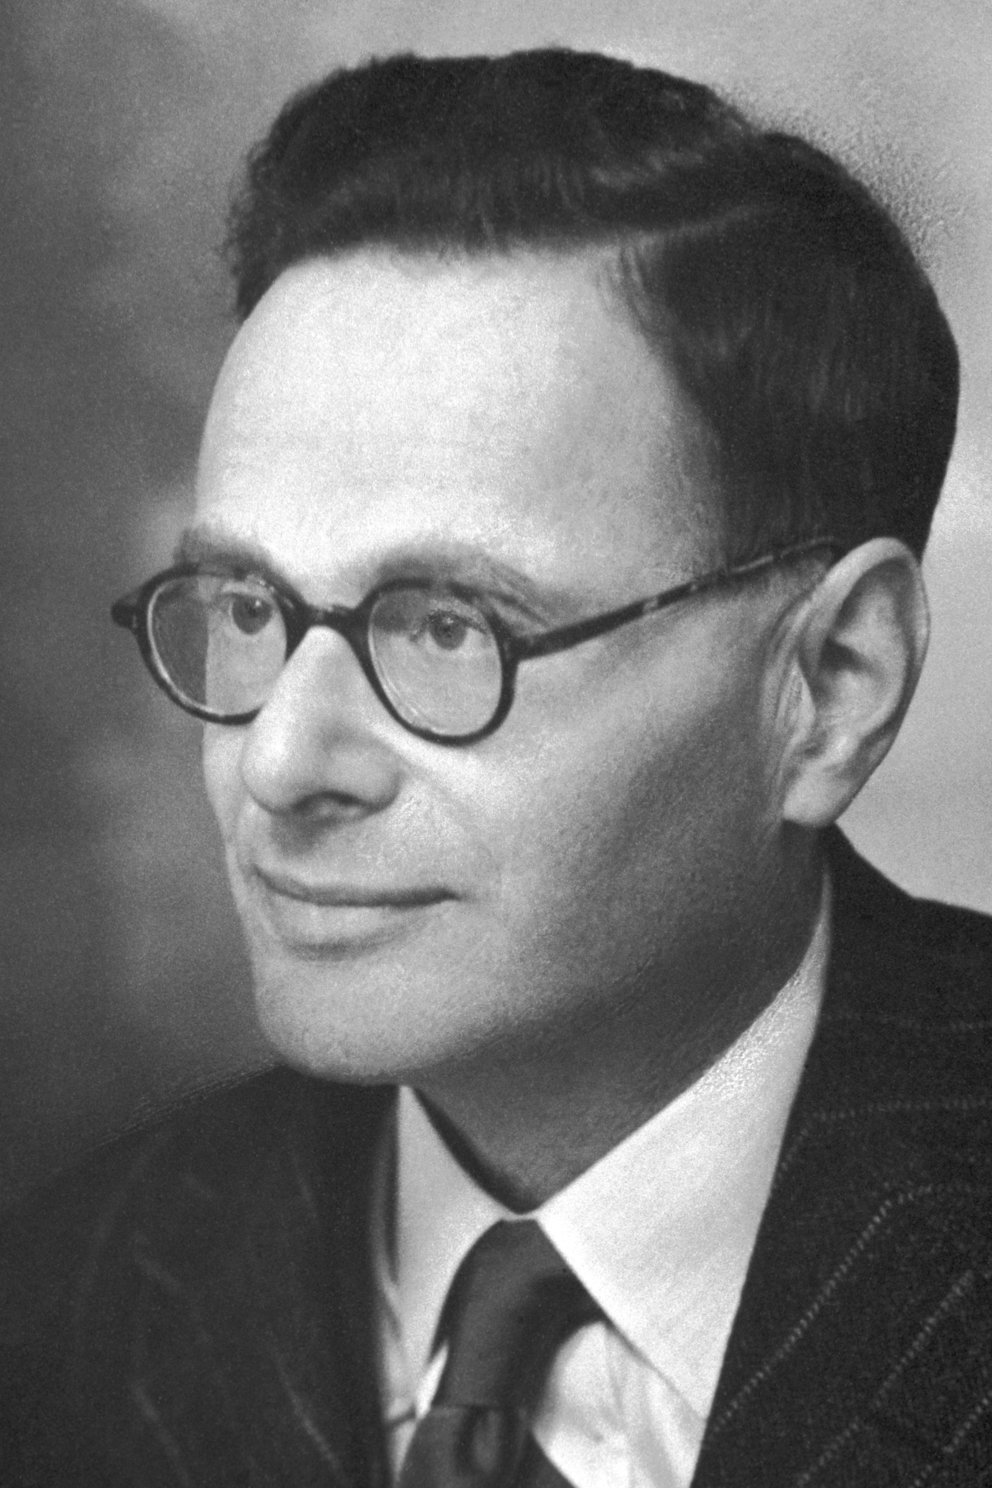
\includegraphics[width=0.26\linewidth]{images/book3/krebs.jpg}

{\small Hans Krebs (1900--1981), que desvendou o ciclo em 1937 a partir
das velocidades com que músculo de pombo moído oxidava os ácidos dele.
Fotografia: Fundação Nobel, domínio público.}
\end{omfigure}

\section{Fosforilação oxidativa}

\begin{definition}[A cadeia respiratória]\label{def:b1:respiration-fermentation:chain}
\index{cadeia respiratória}\index{cadeia transportadora de elétrons}
A \emph{cadeia respiratória} são quatro complexos proteicos da membrana
mitocondrial interna e dois transportadores móveis. O NADH entrega os
elétrons dele ao \emph{complexo I}, e o $\mathrm{FADH_2}$ (pela
succinato-desidrogenase, o \emph{complexo II}) entrega os dele; os dois
reduzem a \emph{ubiquinona} (Q), uma quinona lipossolúvel que se difunde
na membrana; a Q os passa ao \emph{complexo III}, que os entrega ao
\emph{citocromo $c$}, uma \omterm{def:b1:proteins:peptide}{proteína} pequena da face externa; e o
\emph{complexo IV} (a citocromo-oxidase) os entrega, de quatro em
quatro, ao $\mathrm{O_2}$, formando água. Em cada um dos complexos I,
III e IV os elétrons caem em potencial e a energia bombeia prótons da
matriz para o espaço intermembranas: cerca de 4, 4 e 2 por par de
elétrons, dez por NADH e seis por $\mathrm{FADH_2}$ (que entra abaixo do
complexo I).
\end{definition}

\begin{omfigure}
\begin{tikzpicture}[font=\footnotesize, >=Stealth, line cap=round]
  % membrane band
  \fill[omDef!15] (0,0) rectangle (13.0,1.4);
  \draw[omDef!60!black] (0,0) -- (13.0,0) (0,1.4) -- (13.0,1.4);
  \node[anchor=east, gray, align=right] at (-0.15,1.25) {espaço\\ intermembranas\\ (muito $\mathrm{H^+}$, pH 7)};
  \node[anchor=east, gray, align=right] at (-0.15,0.15) {matriz\\ (pouco $\mathrm{H^+}$, pH 8)};
  % complexes
  \node[draw, thick, fill=omThm!25, rounded corners=3pt, minimum height=18mm, minimum width=13mm, align=center] (c1) at (1.5,0.7) {I};
  \node[draw, thick, fill=omThm!25, rounded corners=3pt, minimum height=12mm, minimum width=10mm, align=center] (c2) at (3.6,0.5) {II};
  \node[draw, thick, fill=omThm!25, rounded corners=3pt, minimum height=18mm, minimum width=13mm, align=center] (c3) at (6.2,0.7) {III};
  \node[draw, thick, fill=omThm!25, rounded corners=3pt, minimum height=18mm, minimum width=13mm, align=center] (c4) at (8.9,0.7) {IV};
  \node[draw, thick, fill=omExo!25, rounded corners=6pt, minimum height=16mm, minimum width=12mm, align=center] (atp) at (11.6,0.5) {ATP-\\ sintase};
  \node[circle, draw, thick, fill=omProp!30, inner sep=1.5pt, font=\scriptsize] (q) at (4.9,0.55) {Q};
  \node[circle, draw, thick, fill=omProp!30, inner sep=1.5pt, font=\scriptsize] (cyt) at (7.55,1.25) {cit $c$};
  % electron flow
  \draw[->, thick, omProp] (c1) -- (q); \draw[->, thick, omProp] (c2) -- (q); \draw[->, thick, omProp] (q) -- (c3); \draw[->, thick, omProp] (c3) -- (cyt); \draw[->, thick, omProp] (cyt) -- (c4);
  % inputs
  \node[anchor=north, align=center] at (1.5,-0.5) {NADH $\to$ $\mathrm{NAD^+}$};
  \node[anchor=north, align=center] at (3.6,-0.5) {$\mathrm{FADH_2}$\\ (succinato)};
  \node[anchor=north, align=center, font=\scriptsize] at (8.6,-0.5) {$\tfrac12\,\mathrm{O_2} + 2\,\mathrm{H^+} \to \mathrm{H_2O}$};
  % proton pumping arrows
  \foreach \x/\n in {1.5/4 $\mathrm{H^+}$, 6.2/4 $\mathrm{H^+}$, 8.9/2 $\mathrm{H^+}$} {
    \draw[->, very thick, omExo!80!black] (\x+0.5,-0.05) -- (\x+0.5,1.9) node[above, font=\scriptsize] {\n};
  }
  \draw[->, very thick, omExo!80!black] (11.6,2.1) -- (11.6,1.35);
  \draw[->, very thick, omExo!80!black] (11.6,-0.35) -- (11.6,-0.75);
  \node[anchor=south, font=\scriptsize] at (11.6,2.15) {$\approx 4\,\mathrm{H^+}$/ATP};
  \node[anchor=north, align=center, font=\scriptsize] at (11.6,-0.8) {ADP $+ \mathrm{P_i} \to$ ATP};
\end{tikzpicture}

{\small A membrana mitocondrial interna. Os elétrons (laranja) caem do
NADH ou do $\mathrm{FADH_2}$ pelos complexos até o oxigênio; os
complexos I, III e IV bombeiam prótons para fora (verde); a
\omterm{thm:b1:photosynthesis:chemiosmosis}{ATP-sintase} os deixa voltar e fabrica \omterm{def:b1:water-small-molecules:atp}{ATP}.}
\end{omfigure}

\begin{theorem}[Acoplamento quimiosmótico]\label{thm:b1:respiration-fermentation:chemiosmosis}
\index{teoria quimiosmótica}\index{força próton-motriz}
O gradiente de prótons construído pela cadeia --- cerca de
\qty{0.16}{V} de \omterm{def:b1:membranes-transport:potential}{potencial de membrana} (matriz negativa) mais uma
unidade de pH, uma \emph{\omterm{thm:b1:respiration-fermentation:chemiosmosis}{força próton-motriz}} de cerca de \qty{0.22}{V},
ou \qty{21}{kJ} por mol de prótons --- é o único elo entre o transporte
de elétrons e a síntese de \omterm{def:b1:water-small-molecules:atp}{ATP}. A \omterm{thm:b1:photosynthesis:chemiosmosis}{ATP-sintase}, um motor rotativo da
membrana interna, deixa passar cerca de \qty{3}{H^+} por \omterm{def:b1:water-small-molecules:atp}{ATP} fabricado,
e mais um é gasto para importar o fosfato e exportar o \omterm{def:b1:water-small-molecules:atp}{ATP}: 4 por \omterm{def:b1:water-small-molecules:atp}{ATP}.
Daí a \emph{razão P/O}\index{razão P/O}: $10/4 = 2.5$ \omterm{def:b1:water-small-molecules:atp}{ATP} por NADH e
$6/4 = 1.5$ por $\mathrm{FADH_2}$.
\end{theorem}
\begin{proof}[Evidências]
As \omterm{def:b1:eukaryotic-cell:mitochondrion}{mitocôndrias} só fabricam \omterm{def:b1:water-small-molecules:atp}{ATP} quando a membrana interna delas está
íntegra e fechada; fragmentos que transportam elétrons mas não
conseguem manter um gradiente não fabricam nenhum. Os desacopladores,
como o dinitrofenol, que transportam prótons através da membrana,
abolem a síntese de \omterm{def:b1:water-small-molecules:atp}{ATP} enquanto o consumo de oxigênio continua e até se
acelera, com a energia saindo como calor --- a \omterm{def:b1:lipids:triglyceride}{gordura} marrom faz isso
de propósito com a \omterm{def:b1:proteins:peptide}{proteína} desacopladora dela
(\cref{ch:b1:mammal-organization}), e o dinitrofenol já foi vendido como
remédio para emagrecer que matava por hipertermia. Os \omterm{def:b1:enzymes:inhibitors}{inibidores} da
cadeia (o cianeto sobre o complexo IV) param os dois; os \omterm{def:b1:enzymes:inhibitors}{inibidores} da
sintase (a oligomicina) param a síntese de \omterm{def:b1:water-small-molecules:atp}{ATP} e, com o gradiente sem
poder se descarregar, param também a respiração, que um desacoplador
então restabelece. Um gradiente de pH artificial imposto a \omterm{def:b1:eukaryotic-cell:mitochondrion}{mitocôndrias}
no escuro move a síntese de \omterm{def:b1:water-small-molecules:atp}{ATP}, como nos \omterm{def:b1:eukaryotic-cell:plastid}{cloroplastos}
(\cref{ch:b1:photosynthesis}).
\end{proof}

\begin{omfigure}
\begin{tikzpicture}
  \node[anchor=south west, inner sep=0] (img) at (0,0)
    {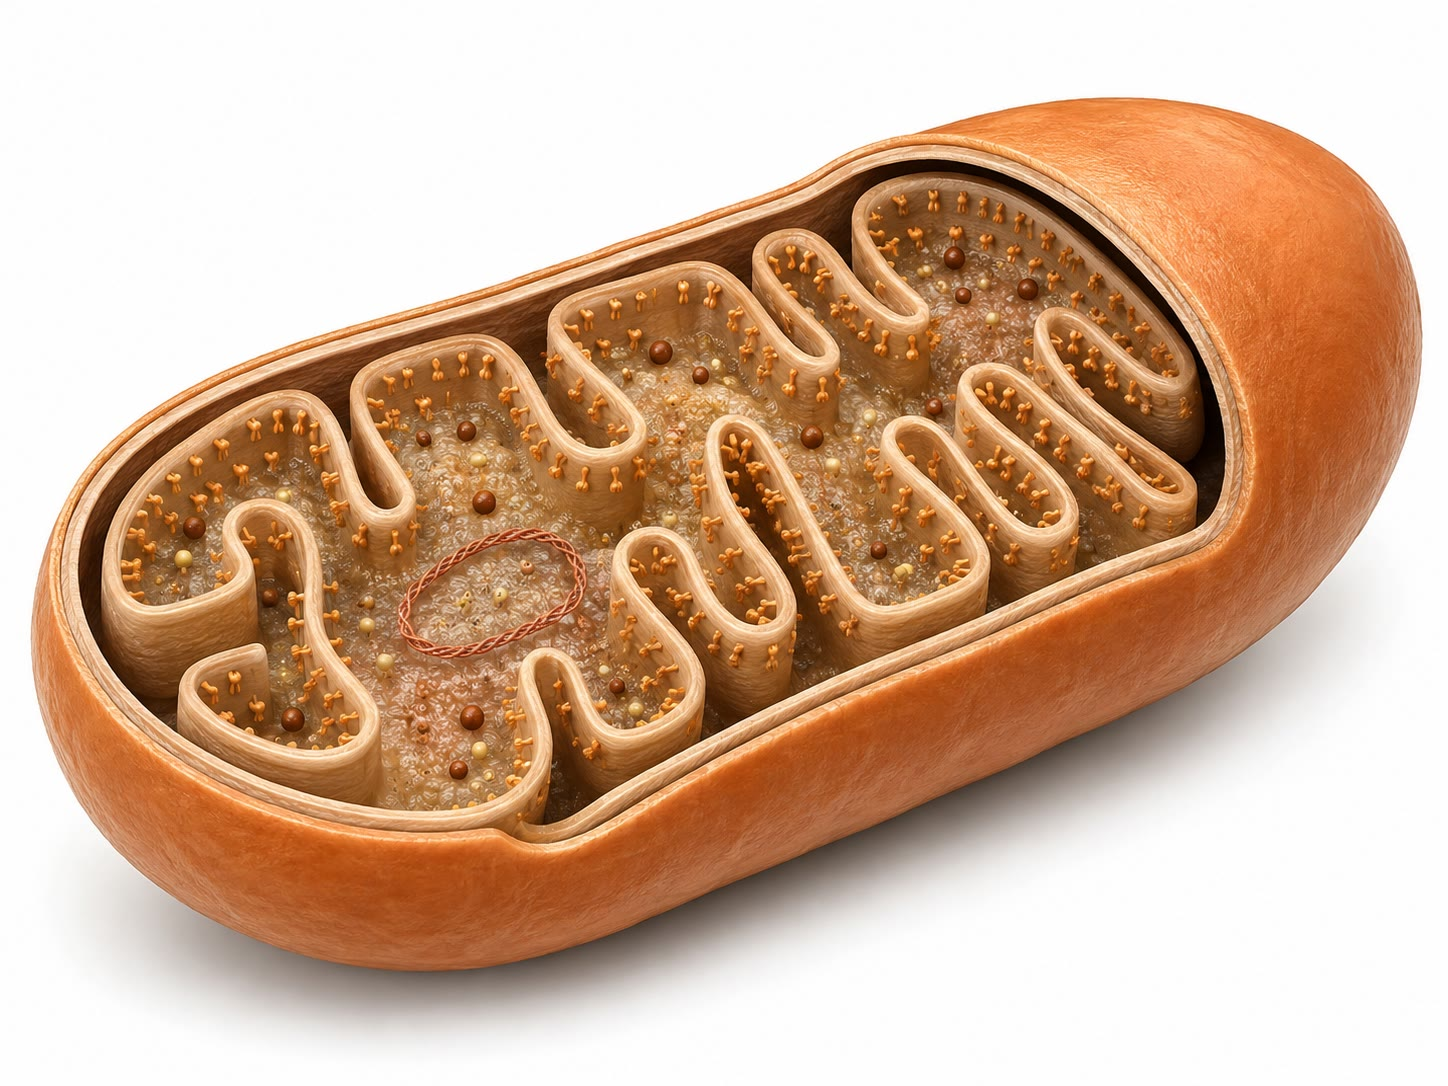
\includegraphics[width=0.54\linewidth]{images/book3/ai/fig-mitochondrion-cutaway.jpg}};
  \begin{scope}[x={(img.south east)}, y={(img.north west)},
      every node/.style={font=\small}]
    \draw[omDef, thick] (0.10,0.55) -- (-0.03,0.70) node[left] {membrana externa};
    \draw[omDef, thick] (0.45,0.72) -- (0.45,1.08) node[above, align=center] {membrana interna dobrada em cristas:\\ a cadeia respiratória\\ e a ATP-sintase};
    \draw[omDef, thick] (0.55,0.35) -- (1.03,0.24) node[right, align=left] {matriz: ciclo\\ de Krebs, DNA,\\ ribossomos};
    \draw[omDef, thick] (0.16,0.40) -- (-0.03,0.26) node[left] {espaço intermembranas};
  \end{scope}
\end{tikzpicture}

{\small Uma \omterm{def:b1:eukaryotic-cell:mitochondrion}{mitocôndria} aberta. As dobras da membrana interna
multiplicam a área disponível para a cadeia e para a sintase; a matriz
lá dentro abriga o \omterm{def:b1:respiration-fermentation:krebs}{ciclo de Krebs}.}
\end{omfigure}

\begin{method}[O balanço de ATP de uma glicose]\label{met:b1:respiration-fermentation:balance}
\begin{enumerate}
  \item \omterm{def:b1:respiration-fermentation:glycolysis}{Glicólise}: $+2$ \omterm{def:b1:water-small-molecules:atp}{ATP} (líquido), $+2$ NADH no \omterm{def:b1:eukaryotic-cell:organelle}{citosol}.
  \item Piruvato-desidrogenase: $+2$ NADH. \omterm{def:b1:respiration-fermentation:krebs}{Ciclo de Krebs}: $+6$ NADH,
        $+2$ $\mathrm{FADH_2}$, $+2$ GTP ($=$ \omterm{def:b1:water-small-molecules:atp}{ATP}).
  \item Fosforilação oxidativa: $2.5$ \omterm{def:b1:water-small-molecules:atp}{ATP} por NADH mitocondrial (8: 20
        \omterm{def:b1:water-small-molecules:atp}{ATP}), $1.5$ por $\mathrm{FADH_2}$ (2: 3 \omterm{def:b1:water-small-molecules:atp}{ATP}).
  \item O NADH citosólico não atravessa a membrana interna; os elétrons
        dele entram por uma lançadeira que os entrega ao $\mathrm{FAD}$
        (1.5 cada, no músculo e no encéfalo) ou ao $\mathrm{NAD^+}$ (2.5
        cada, no fígado e no coração): 3 ou 5 \omterm{def:b1:water-small-molecules:atp}{ATP}.
  \item Total: $2 + 2 + 20 + 3 + 3 = 30$, ou $32$ com a lançadeira
        melhor. Eficiência: $30\times 50/2870 \approx \qty{52}{\%}$ nas
        condições celulares.
\end{enumerate}
\end{method}

\section{Fermentação}

\begin{definition}[Fermentação]\label{def:b1:respiration-fermentation:fermentation}
\index{fermentação}
Sem oxigênio a \omterm{def:b1:respiration-fermentation:chain}{cadeia respiratória} para, o NADH não pode ser reoxidado,
e a \omterm{def:b1:respiration-fermentation:glycolysis}{glicólise} pararia em poucos segundos por falta de
$\mathrm{NAD^+}$. A \emph{fermentação} o regenera usando o próprio
piruvato como aceptor de elétrons: na \emph{fermentação láctica}
(músculo, hemácias, bactérias lácticas) o piruvato é reduzido a
lactato; na \emph{fermentação alcoólica} (leveduras, algumas plantas)
ele é descarboxilado a acetaldeído, que é reduzido a etanol, liberando
$\mathrm{CO_2}$. O rendimento é o da própria \omterm{def:b1:respiration-fermentation:glycolysis}{glicólise}: 2 \omterm{def:b1:water-small-molecules:atp}{ATP} por
glicose, um quinze avos do da respiração; o carbono é pouquíssimo
oxidado e os produtos ainda guardam quase toda a energia do combustível.
A \emph{respiração anaeróbia} --- uma cadeia de transporte de elétrons
que termina em nitrato, sulfato ou carbonato em vez de oxigênio, em
muitas bactérias --- é outra coisa, tratada no volume do Ano 2.
\end{definition}

\begin{omfigure}
\begin{minipage}[b]{0.44\linewidth}\centering
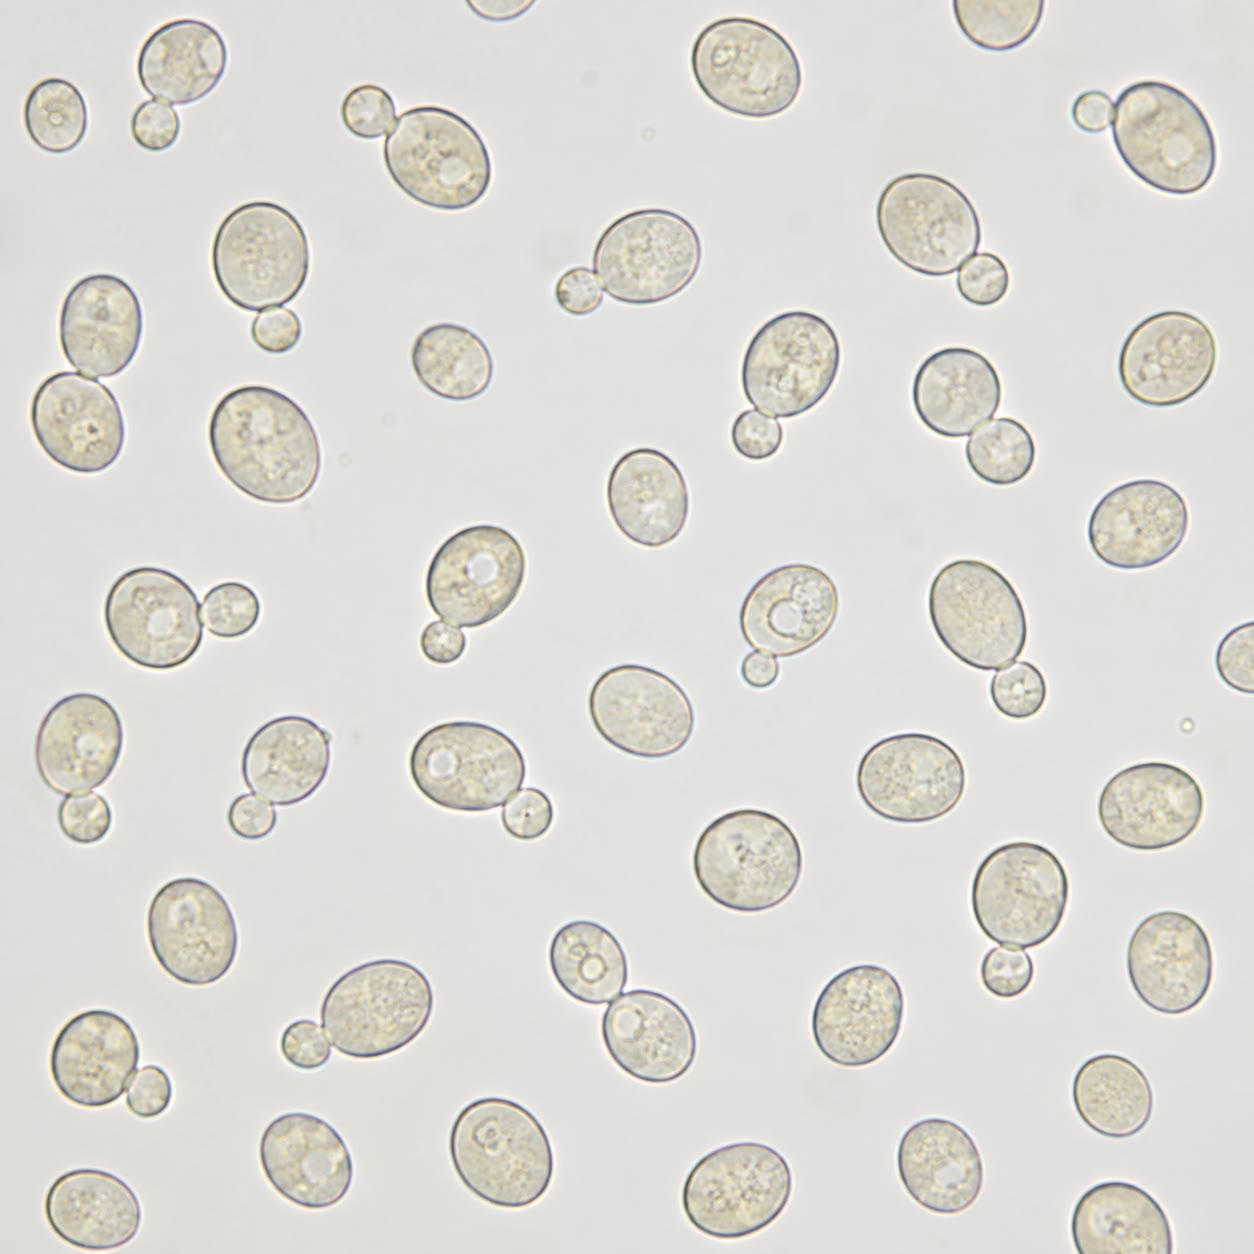
\includegraphics[width=0.9\linewidth]{images/book3/ai/b3-15-yeast-budding.jpg}
\end{minipage}\hfill
\begin{minipage}[b]{0.52\linewidth}\centering
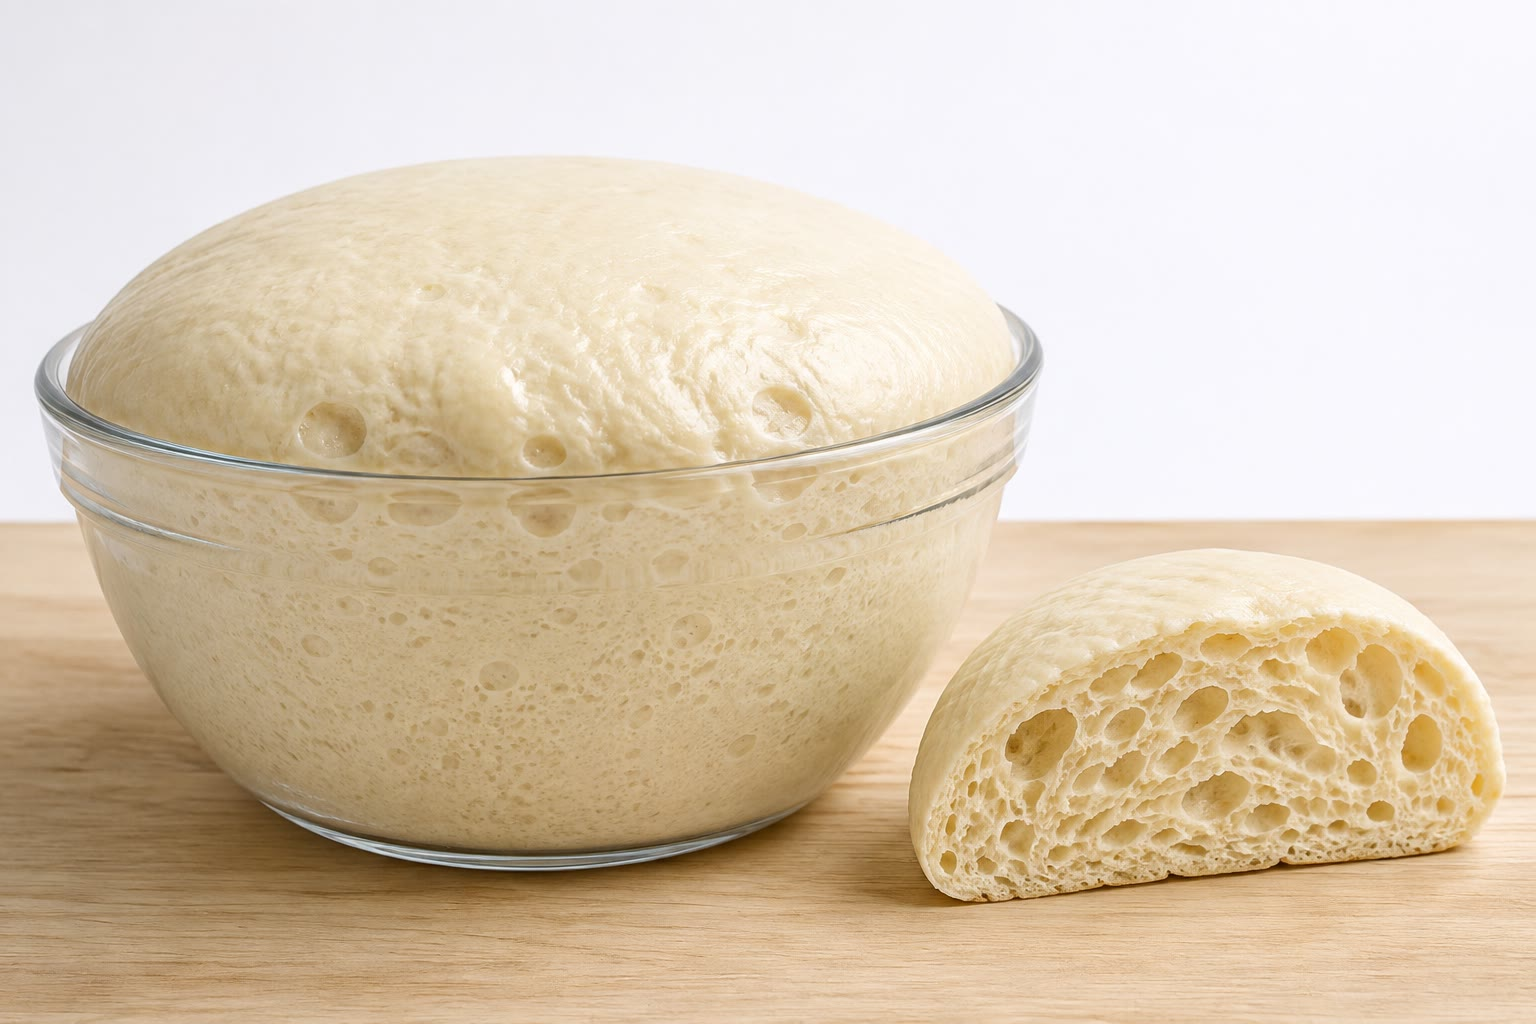
\includegraphics[width=0.96\linewidth]{images/book3/ai/b3-15-bread-dough-risen.jpg}
\end{minipage}

{\small À esquerda: levedura de padeiro, brotando. À direita: o que a
\omterm{def:b1:respiration-fermentation:fermentation}{fermentação} dela faz com a massa: o $\mathrm{CO_2}$ de dois \omterm{def:b1:water-small-molecules:atp}{ATP} de
\omterm{def:b1:respiration-fermentation:glycolysis}{glicólise} por glicose, preso no glúten. O etanol evapora no forno.}
\end{omfigure}

\begin{proposition}[O efeito Pasteur]\label{prop:b1:respiration-fermentation:pasteur}
\index{efeito Pasteur}
Uma \omterm{def:b1:cell-unit-of-life:cell}{célula} capaz de respirar consome glicose muito mais depressa quando
privada de oxigênio do que quando ele é fornecido, e cresce muito menos
com ela.
\end{proposition}
\begin{proof}[Evidências]
Pasteur (1861) viu a levedura de uma cuba arejada consumindo açúcar
devagar e se multiplicando, ao passo que numa cuba selada ela consumia
açúcar dez vezes mais depressa, multiplicava-se pouco e fabricava
álcool. A explicação é o rendimento de \omterm{def:b1:water-small-molecules:atp}{ATP}: para obter o mesmo \omterm{def:b1:water-small-molecules:atp}{ATP} a
partir de 2 por glicose em vez de 30, a \omterm{def:b1:cell-unit-of-life:cell}{célula} precisa rodar a \omterm{def:b1:respiration-fermentation:glycolysis}{glicólise}
quinze vezes mais rápido, e a PFK, liberada da inibição pelo \omterm{def:b1:water-small-molecules:atp}{ATP} e pelo
citrato que a respiração mantém, permite isso. Um músculo em disparada
mostra o mesmo efeito em poucos segundos: o \omterm{def:b1:carbohydrates:polysaccharide}{glicogênio} dele cai vinte
vezes mais depressa que em repouso, e o lactato sobe.
\end{proof}

\begin{definition}[Quociente respiratório]\label{def:b1:respiration-fermentation:rq}
\index{quociente respiratório}
O \emph{quociente respiratório} QR é a razão entre o $\mathrm{CO_2}$
produzido e o $\mathrm{O_2}$ consumido, em mols. O \omterm{def:b1:carbohydrates:monosaccharide}{carboidrato} dá 1.0
(seis de cada por glicose); a \omterm{def:b1:lipids:triglyceride}{gordura}, cerca de 0.7 (palmitato:
$\mathrm{C_{16}H_{32}O_2} + 23\,\mathrm{O_2} \to 16\,\mathrm{CO_2} +
16\,\mathrm{H_2O}$, $16/23 = 0.70$), porque os carbonos dela são mais
reduzidos e precisam de mais oxigênio por $\mathrm{CO_2}$; a \omterm{def:b1:proteins:peptide}{proteína},
cerca de 0.8. Uma cultura em \omterm{def:b1:respiration-fermentation:fermentation}{fermentação} libera $\mathrm{CO_2}$ sem
captar oxigênio: o QR dela é infinito, e um QR acima de 1 numa cultura
mista mede a parcela de \omterm{def:b1:respiration-fermentation:fermentation}{fermentação}. Medido num animal inteiro por
análise dos gases, o QR diz qual combustível ele está queimando.
\end{definition}

\begin{example}[Ler um QR]\label{ex:b1:respiration-fermentation:readrq}
Um ser humano em repouso depois de uma refeição rica em \omterm{def:b1:carbohydrates:monosaccharide}{carboidratos}: QR
0.95, queimando glicose. A mesma pessoa depois de uma noite de jejum:
0.75, \omterm{def:b1:lipids:triglyceride}{gordura}. Um maratonista no trigésimo quilômetro, com o \omterm{def:b1:carbohydrates:polysaccharide}{glicogênio}
esgotado: 0.72. Um frasco de levedura em glicose com um pouco de ar: QR
4 --- três quartos da glicose dela estão sendo fermentados.
\end{example}

\section{Outros combustíveis e a regulação do conjunto}

\begin{proposition}[As gorduras e as proteínas entram na mesma maquinaria]\label{prop:b1:respiration-fermentation:otherfuels}
\index{beta-oxidacao@$\beta$-oxidação}
Os \omterm{def:b1:lipids:fattyacid}{ácidos graxos} são ativados a acil-CoA e, na \omterm{def:b1:eukaryotic-cell:mitochondrion}{matriz mitocondrial},
encurtados de dois em dois carbonos pela \emph{$\beta$-oxidação}, com
cada rodada rendendo um \omterm{def:b1:respiration-fermentation:pdh}{acetil-CoA}, um NADH e um $\mathrm{FADH_2}$: o
palmitato (C16) dá 8 \omterm{def:b1:respiration-fermentation:pdh}{acetil-CoA}, 7 NADH e 7 $\mathrm{FADH_2}$ --- cerca
de 106 \omterm{def:b1:water-small-molecules:atp}{ATP}, ou \qty{6.6}{} \omterm{def:b1:water-small-molecules:atp}{ATP} por carbono contra os 5 da glicose. Os
\omterm{def:b1:proteins:aminoacid}{aminoácidos} perdem o nitrogênio deles como amônia (convertida em ureia
no fígado) e os esqueletos de carbono deles entram como piruvato,
\omterm{def:b1:respiration-fermentation:pdh}{acetil-CoA} ou intermediários do \omterm{def:b1:respiration-fermentation:krebs}{ciclo de Krebs}. Todo combustível
converge para o \omterm{def:b1:respiration-fermentation:pdh}{acetil-CoA} e para a cadeia; a \omterm{def:b1:cell-unit-of-life:cell}{célula} escolhe entre eles
por hormônios e pelo estado do \omterm{def:b1:water-small-molecules:atp}{ATP} dela, como descreve o
\cref{ch:b1:biosyntheses-integration}.
\end{proposition}

\begin{example}[Um grama de cada]\label{ex:b1:respiration-fermentation:gramofeach}
Um grama de glicose (\qty{5.6}{mmol}) rende cerca de \qty{170}{mmol} de
\omterm{def:b1:water-small-molecules:atp}{ATP}; um grama de palmitato (\qty{3.9}{mmol}), cerca de \qty{410}{mmol}
--- os \qty{38}{kJ/g} contra os \qty{17}{kJ/g} do \cref{ch:b1:lipids},
convertidos em moeda. A \omterm{def:b1:lipids:triglyceride}{gordura} custa mais oxigênio por \omterm{def:b1:water-small-molecules:atp}{ATP}, e é por
isso que o músculo de um velocista, limitado pelo oxigênio, queima
\omterm{def:b1:carbohydrates:polysaccharide}{glicogênio}, e uma ave migratória, com oxigênio de sobra e limitada pela
massa, queima \omterm{def:b1:lipids:triglyceride}{gordura}.
\end{example}

\section{Exercícios}

\begin{exercise}[$\star$]\label{exo:b1:respiration-fermentation:1}
Cite as três etapas da respiração, a localização delas e o que cada uma
produz.
\end{exercise}

\begin{exercise}[$\star$]\label{exo:b1:respiration-fermentation:2}
Escreva o balanço da \omterm{def:b1:respiration-fermentation:glycolysis}{glicólise} e explique a ``\omterm{def:b1:respiration-fermentation:glycolysis}{fosforilação em nível de
substrato}''.
\end{exercise}

\begin{exercise}[$\star$]\label{exo:b1:respiration-fermentation:3}
A partir da figura do \omterm{def:b1:respiration-fermentation:krebs}{ciclo de Krebs}, liste em ordem os produtos
liberados em uma volta, e diga de onde vêm os dois $\mathrm{CO_2}$.
\end{exercise}

\begin{exercise}[$\star$]\label{exo:b1:respiration-fermentation:4}
O que a \omterm{def:b1:respiration-fermentation:fermentation}{fermentação} realiza para uma \omterm{def:b1:cell-unit-of-life:cell}{célula} sem oxigênio, e o que ela
não realiza?
\end{exercise}

\begin{exercise}[$\star\star$]\label{exo:b1:respiration-fermentation:5}
Calcule o $\Delta G^{\circ\prime}$ da transferência de dois elétrons do
NADH ($E'_0 = \qty{-0.32}{V}$) para o oxigênio (\qty{+0.82}{V}) e para
a ubiquinona (\qty{+0.05}{V}). Quantos \omterm{def:b1:water-small-molecules:atp}{ATP} cada etapa poderia pagar, em
princípio?
\end{exercise}

\begin{exercise}[$\star\star$]\label{exo:b1:respiration-fermentation:6}
Monte o balanço de \omterm{def:b1:water-small-molecules:atp}{ATP} de uma glicose numa \omterm{def:b1:cell-unit-of-life:cell}{célula} muscular (lançadeira
do glicerol-fosfato) e numa \omterm{def:b1:cell-unit-of-life:cell}{célula} do fígado (lançadeira do malato),
usando \omterm{thm:b1:respiration-fermentation:chemiosmosis}{razões P/O} de 2.5 e 1.5.
\end{exercise}

\begin{exercise}[$\star\star$]\label{exo:b1:respiration-fermentation:7}
Uma cultura consome \qty{1.0}{mmol} de $\mathrm{O_2}$ e libera
\qty{2.2}{mmol} de $\mathrm{CO_2}$ por hora em glicose. Calcule o QR e
as frações da glicose respirada e fermentada.
\end{exercise}

\begin{exercise}[$\star\star$]\label{exo:b1:respiration-fermentation:8}
Explique o que acontece com o consumo de oxigênio, com a síntese de \omterm{def:b1:water-small-molecules:atp}{ATP}
e com a produção de calor quando se acrescenta dinitrofenol a
\omterm{def:b1:eukaryotic-cell:mitochondrion}{mitocôndrias} em respiração, e por que a droga era letal.
\end{exercise}

\begin{exercise}[$\star\star$]\label{exo:b1:respiration-fermentation:9}
O cianeto bloqueia o complexo IV. Preveja o efeito dele sobre a \omterm{def:b1:respiration-fermentation:chain}{cadeia
respiratória}, sobre o \omterm{def:b1:respiration-fermentation:krebs}{ciclo de Krebs} e sobre a \omterm{def:b1:respiration-fermentation:glycolysis}{glicólise} numa \omterm{def:b1:cell-unit-of-life:cell}{célula}, e
explique por que o lactato se acumula no sangue de quem foi envenenado.
\end{exercise}

\begin{exercise}[$\star\star\star$]\label{exo:b1:respiration-fermentation:10}
Calcule o rendimento em \omterm{def:b1:water-small-molecules:atp}{ATP} do palmitato (8 \omterm{def:b1:respiration-fermentation:pdh}{acetil-CoA}, 7 NADH, 7
$\mathrm{FADH_2}$, menos 2 \omterm{def:b1:water-small-molecules:atp}{ATP} da ativação) e o rendimento por carbono;
calcule o oxigênio consumido por \omterm{def:b1:water-small-molecules:atp}{ATP} para o palmitato e para a glicose.
Que combustível uma foca mergulhadora deveria preferir, e qual um
beija-flor?
\end{exercise}

\begin{exercise}[$\star\star\star$]\label{exo:b1:respiration-fermentation:11}
Uma fibra muscular contém \qty{5}{mmol/L} de \omterm{def:b1:water-small-molecules:atp}{ATP} e usa
\qty{3}{mmol/L} por segundo numa disparada. Quanto tempo o \omterm{def:b1:water-small-molecules:atp}{ATP} dela
duraria sozinho? A fosfocreatina dela (\qty{25}{mmol/L}) regenera \omterm{def:b1:water-small-molecules:atp}{ATP} um
por um; o \omterm{def:b1:carbohydrates:polysaccharide}{glicogênio} dela, pela \omterm{def:b1:respiration-fermentation:fermentation}{fermentação}, dá 3 \omterm{def:b1:water-small-molecules:atp}{ATP} por unidade de
glicose, a até \qty{2}{mmol/L} de unidades de glicose por segundo.
Calcule o tempo que cada reserva consegue sustentar a disparada e
explique por que uma prova de 100 m é corrida quase inteiramente sem
oxigênio.
\end{exercise}

\begin{exercise}[$\star\star\star$]\label{exo:b1:respiration-fermentation:12}
``A \omterm{def:b1:eukaryotic-cell:mitochondrion}{mitocôndria} é uma bateria carregada por elétrons e descarregada por
uma turbina.'' Discuta em um parágrafo: o que o gradiente armazena, o
que a sintase faz, onde a analogia é exata e onde ela é frouxa.
\end{exercise}

\section{Problema: Levedura com ar e sem ar}

\begin{problem}[{Problema de fim de semana --- as cubas de Pasteur
revisitadas: ATP contado, glicose consumida, biomassa produzida e gases
medidos, terminando na razão entre os rendimentos de ATP e na razão P/O}]
\label{pb:b1:respiration-fermentation:1}
Levedura é cultivada em glicose em dois frascos idênticos, um arejado e
um selado. Use \omterm{thm:b1:respiration-fermentation:chemiosmosis}{razões P/O} de 2.5 (NADH) e 1.5 ($\mathrm{FADH_2}$), a
lançadeira do $\mathrm{FADH_2}$ para o NADH citosólico, um rendimento de
crescimento de \qty{10.5}{g} de biomassa seca por mol de \omterm{def:b1:water-small-molecules:atp}{ATP}, e glicose
a \qty{180}{g/mol}.

\medskip
\noindent\textbf{Parte I --- \omterm{def:b1:water-small-molecules:atp}{ATP} contado.}
\begin{enumerate}
  \item Liste o \omterm{def:b1:water-small-molecules:atp}{ATP}, o GTP, o NADH e o $\mathrm{FADH_2}$ produzidos a
        partir de uma glicose pela \omterm{def:b1:respiration-fermentation:glycolysis}{glicólise}, pela
        piruvato-desidrogenase e pelo \omterm{def:b1:respiration-fermentation:krebs}{ciclo de Krebs}.
  \item Calcule os prótons bombeados pela cadeia por glicose (10 por
        NADH mitocondrial, 6 por $\mathrm{FADH_2}$; o NADH citosólico
        entra como $\mathrm{FADH_2}$).
  \item Calcule o \omterm{def:b1:water-small-molecules:atp}{ATP} fabricado pela sintase a \qty{4}{H^+} por \omterm{def:b1:water-small-molecules:atp}{ATP}, e o
        \omterm{def:b1:water-small-molecules:atp}{ATP} total por glicose com ar.
  \item Calcule o \omterm{def:b1:water-small-molecules:atp}{ATP} por glicose sem ar.
  \item Calcule a razão entre os dois rendimentos.
  \item Calcule a \omterm{prop:b1:water-small-molecules:gibbs}{energia livre} capturada com ar ($\Delta G_{\text{ATP}}
        = \qty{-50}{kJ/mol}$) como fração dos \qty{2870}{kJ}, e sem ar
        como fração dos \qty{2870}{kJ} e da energia de fato liberada
        pela \omterm{def:b1:respiration-fermentation:fermentation}{fermentação} (glicose a dois etanóis e dois
        $\mathrm{CO_2}$: \qty{-235}{kJ/mol}).
\end{enumerate}

\medskip
\noindent\textbf{Parte II --- Glicose consumida, biomassa produzida.}
O frasco selado precisa fabricar \omterm{def:b1:water-small-molecules:atp}{ATP} à mesma velocidade que o arejado
para manter as \omterm{def:b1:cell-unit-of-life:cell}{células} dele: \qty{30}{mmol} de \omterm{def:b1:water-small-molecules:atp}{ATP} por hora.
\begin{enumerate}[resume]
  \item Calcule a glicose consumida por hora em cada frasco.
  \item Calcule o etanol e o $\mathrm{CO_2}$ produzidos por hora no
        frasco selado, e o $\mathrm{CO_2}$ e o $\mathrm{O_2}$ trocados
        no arejado.
  \item Calcule a biomassa que o frasco selado consegue construir por
        mol de glicose e por grama de glicose.
  \item O frasco arejado constrói \qty{0.5}{g} de biomassa por grama de
        glicose. Calcule o \omterm{def:b1:water-small-molecules:atp}{ATP} que isso representaria a
        \qty{10.5}{g/mol}, e compare com os 30 \omterm{def:b1:water-small-molecules:atp}{ATP} disponíveis. O que
        limita o rendimento aeróbio?
  \item Explique o \omterm{prop:b1:respiration-fermentation:pasteur}{efeito Pasteur} a partir das questões 7 e 9, e cite a
        \omterm{def:b1:enzymes:enzyme}{enzima} cuja regulação o implementa.
\end{enumerate}

\medskip
\noindent\textbf{Parte III --- Gases medidos.}
Um terceiro frasco, mal arejado, libera \qty{44}{mg} de $\mathrm{CO_2}$
e consome \qty{20}{mg} de $\mathrm{O_2}$ por hora.
\begin{enumerate}[resume]
  \item Converta os dois em milimols e calcule o QR.
  \item Seja $x$ a glicose respirada e $y$ a glicose fermentada por
        hora. Escreva os balanços de $\mathrm{O_2}$ e de
        $\mathrm{CO_2}$ e resolva para $x$ e $y$.
  \item Que fração da glicose é fermentada? Que fração do \omterm{def:b1:water-small-molecules:atp}{ATP} vem da
        \omterm{def:b1:respiration-fermentation:fermentation}{fermentação}?
  \item O mesmo frasco em palmitato no lugar da glicose (em aerobiose):
        calcule o QR.
  \item Um estudante mede um QR de 0.7 num animal em repouso depois de
        uma noite de jejum e de 1.0 depois de uma refeição. Interprete.
\end{enumerate}

\medskip
\noindent\textbf{Parte IV --- A turbina.}
\begin{enumerate}[resume]
  \item Calcule a \omterm{prop:b1:water-small-molecules:gibbs}{energia livre} de um mol de prótons que atravessa uma
        \omterm{thm:b1:respiration-fermentation:chemiosmosis}{força próton-motriz} de \qty{0.22}{V}.
  \item Calcule a energia de \qty{4}{H^+} e a eficiência da sintase a
        \qty{50}{kJ} por \omterm{def:b1:water-small-molecules:atp}{ATP}.
  \item Calcule a \omterm{prop:b1:water-small-molecules:gibbs}{energia livre} liberada por dois elétrons que caem do
        NADH ao $\mathrm{O_2}$ (\qty{1.14}{V}), a energia armazenada nos
        dez prótons bombeados, e a eficiência da cadeia.
  \item Combine as duas eficiências e compare com 2.5 \omterm{def:b1:water-small-molecules:atp}{ATP} $\times$
        \qty{50}{kJ} sobre \qty{220}{kJ}.
  \item Um desacoplador é acrescentado ao frasco arejado. Preveja as
        mudanças no consumo de oxigênio, no rendimento de \omterm{def:b1:water-small-molecules:atp}{ATP}, no
        consumo de glicose, na produção de calor e no crescimento.
  \item A oligomicina, que bloqueia a sintase, é acrescentada em vez
        dele. Preveja as mudanças, e o que acontece se um desacoplador
        for acrescentado por cima.
  \item Uma levedura mutante não tem o complexo I; o NADH dela entra na
        cadeia por uma \omterm{def:b1:enzymes:enzyme}{enzima} alternativa que não bombeia prótons.
        Calcule a \omterm{thm:b1:respiration-fermentation:chemiosmosis}{razão P/O} dela para o NADH e o \omterm{def:b1:water-small-molecules:atp}{ATP} por glicose dela.
  \item Explique por que a \omterm{def:b1:cell-unit-of-life:cell}{célula} mantém o estoque de NADH mitocondrial
        quase todo reduzido quando falta oxigênio, e o que isso faz com
        o \omterm{def:b1:respiration-fermentation:krebs}{ciclo de Krebs}.
  \item Enuncie o resultado: o \omterm{def:b1:water-small-molecules:atp}{ATP} por glicose com ar e sem ar, a razão
        entre os dois, e as \omterm{thm:b1:respiration-fermentation:chemiosmosis}{razões P/O} do NADH e do $\mathrm{FADH_2}$.
\end{enumerate}
\end{problem}
